\documentclass{article}

\usepackage[utf8]{inputenc}
\usepackage{graphicx} % Comandos para manejar imágenes
\graphicspath{ {./images/} } % Carpeta de imágenes

\setlength{\parskip}{2mm} % Espaciado

\usepackage[utf8]{inputenc}
\usepackage{geometry}
    \geometry{left=3cm,right=2cm,top=2cm,bottom=2cm}
%
\usepackage[spanish]{babel}
%
\usepackage[fixlanguage]{babelbib}
    \bibliographystyle{babunsrt}
%

\usepackage{floatrow}
\floatsetup[table]{style=plaintop}

\usepackage{url}

\usepackage[top=2cm, bottom=2.5cm, right=3 cm, left=3 cm]{geometry} % margenes

\usepackage{parskip} % Sangria

\title{Seminario cuatro: ¿Qué son los repuestos críticos y por qué nos importan tanto? comentarios sobre la presentación del Doctor Orlando Durán}
\author{Cristóbal Galleguillos Ketterer$^{1}$\\
\small{$^{1}$Industrial PhD Program}\\
\small{Pontificia Universidad Católica de Valparaíso}\\
\small{cristobal.galleguillos@pucv.cl}
}
\date{\small{\today}}

\begin{document}

\maketitle

\section{Introducción}

Una pala es un equipo de grandes dimensiones, que tiene como objetivo extraer el material (sólidos minerales) para un posterior procesamiento mecánico y químico. Por cada unidad de masa de ese material, encontraremos al final del proceso un porcentaje de cobre, plata, oro y molibdeno, los cuales serán comercializados alrededor del mundo.  Un segundo de detención de la pala implica una cantidad de masa que no se extraer y por lo tanto, cobre, plata y oro que no se puede vender. El equipo está detenido porque una válvula de menos de 100 USD falló y está en el área de mantención mina, distante a 43 kilómetros del rajo (lugar de extracción de material a cielo abierto)

¿Cuál es el costo social y económico de que una línea de packing de manzanas tenga que detenerse por una semana a causa de la demora de un set de rodamientos?

Una turbina a vapor percibe ingresos del Sistema Eléctrico Nacional por energía suministrada y potencia conectada, si uno de los sellos falla (elastómeros que garantizan la estanquidad entre dos espacios), causaría una detención mayor, un cambio del sello. Y, ¿si el sello no está en bodega?, ¿hay que importarlo?, ¿si la detención se alarga y es un año de sequía?

Parece ser un asunto lleno de incertidumbres, bodegas, costos, demoras. En esta tarea presentaremos brevemente los trabajos del doctor Durán sobre estimación y optimización de la gestión de repuestos críticos.



\subsection{Alcance}

La contribución del doctor Durán se presentará desde el punto de vista del desarrollo del modelo costos, las extenciones a este modelo solo serán mencionadas.

\section{Revisión de la literatura}

En esta ocasión analizaremos la literatura generada en función del aporte del autor, en este caso, el Doctor Duran, de este modo podremos obtener otras aristas del análisis bibliográfico.

El trabajo del profesor Duran se fundamenta en el desarrollo de modelos matemáticos de optimización y metaheurísticos como la \textit{particle swarm optimization} un zoom al mapa de las relaciones complejas de información de estas investigaciones se presenta en la Figura \ref{meta}

\begin{figure}[H]
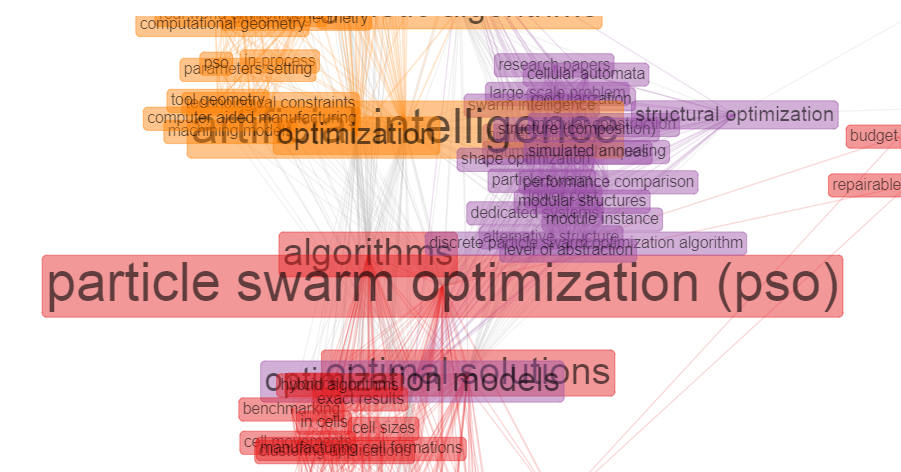
\includegraphics[scale=0.6]{Images/meta.png}
\centering
\caption{Zoom a red compleja de conceptos}
\label{meta}
\end{figure}

La Figura \ref{arbol} representa el mapa de los conceptos comúnmente utilizadas en la investigación científica asociada al estudio del autor, en él destaca ampliamente el campo de la ingeniería mecánica y la ingeniería industrial.

\begin{figure}[H]
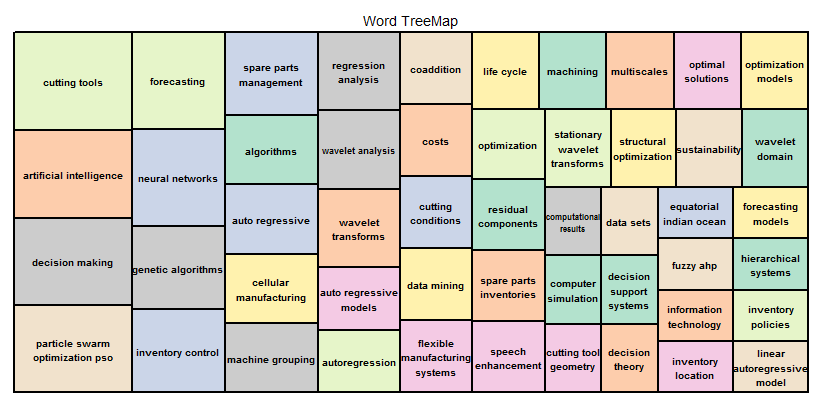
\includegraphics[scale=0.5]{Images/arbol.png}
\centering
\caption{Árbol de conceptos}
\label{arbol}
\end{figure}

Como investigador, resulta interesante conocer las principales fuentes que utiliza el profesor Durán en su investigación, es de interés para considerar las publicaciones que son relevantes en su campo de estudio e identificar el impacto de ellas en el ambiente científico (ver Figura \ref{jo}).

\begin{figure}[H]
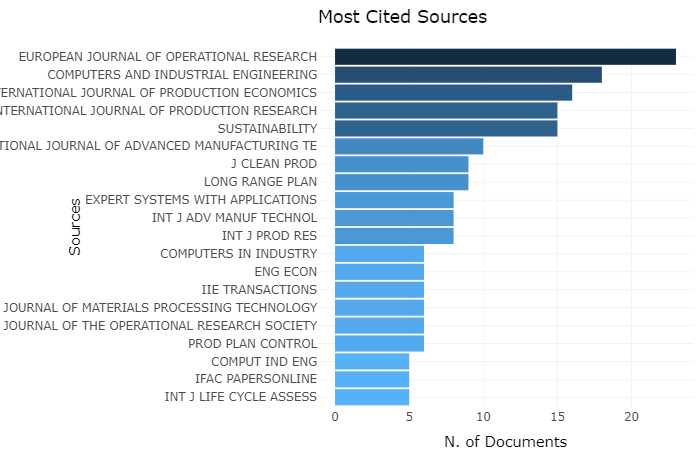
\includegraphics[scale=0.5]{Images/newplot (5).png}
\centering
\caption{Fuentes más citadas}
\label{jo}
\end{figure}

Otro aspecto relevante, a considerar, es la interacción de los científicos y la colaboración en la producción que se da, ya sea de forma transnacional o transcontinental. Este intercambio permite apreciar de que modo las instituciones y los campos del conocimiento están conectados y como la convergencia de diversas experiencias (y culturas, y costumbres) inciden en la investigación científica. En el caso del autor podemos observar el mapa de relaciones de la Figura \ref{mapa}.

\begin{figure}[H]
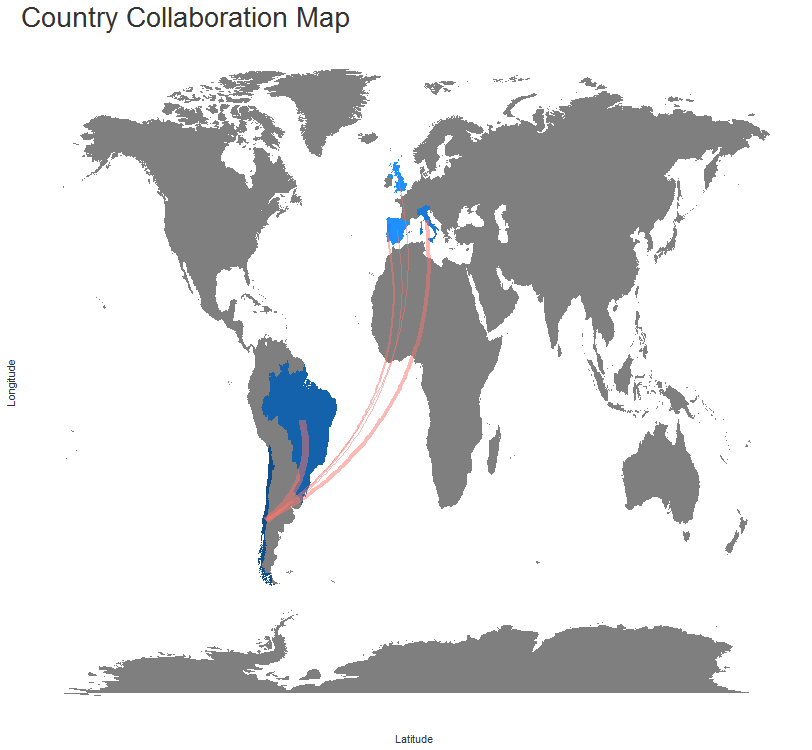
\includegraphics[scale=0.4]{Images/MapaCola.png}
\centering
\caption{Mapa de colaboraciones}
\label{mapa}
\end{figure}

\section{Marco teórico}

El mantenimiento es una de las sub disciplinas de la ingeniería mecánica e industrial, que mas relevancia a ido tomando en la gestión de las industrial con más vigencia en la actualidad, y una de las más demandantes desde el punto de vista laboral/operacional, como en el ámbito de la investigación aplicada.

En términos generales el mantenimiento es un problema económico donde el agente debe decidir cuanto invertir, de acuerdo al tipo de mantenimiento podemos definir en términos generales (tomado parcialmente de \cite{lib1:T1})

\begin{enumerate}

\item \textbf{Mantenimiento correctivo (o a la falla)}: En este caso los componentes son mantenidos tras su falla, las actividades no son planificadas y se pueden lograr ahorros en función de carecer de una estructura formal dedicada a la mantención.
\item \textbf{Mantenimiento Preventivo}: Los componentes son identificados en base a la unidad mínima mantenible, agrupados por criticidad y definidas las actividades y frecuencias de las actividades de mantenimiento, las actividades son planificadas lo que incide en los costos operativos, adicionalmente requiere de mayor infraestructura profesional, de equipamiento y repuestos.
\item \textbf{Mantenimiento Predictivo}: Se basa en el monitoreo de ciertas condiciones (vibraciones, ruidos, temperaturas, análisis de lubricantes) que permiten anticipar los deterioros de un componente que puedan afectar el desempeño del equipo. Es un tipo de mantenimiento con un alto costo de implementación, por la instalación de sensores y el manejo de datos, su venta es que puede anticipar fallas operacionales y garantiza una mayor continuidad operacional.
 \end{enumerate}

Un componente o repuesto, es un activo físico de la empresa, que forma parque de un equipo o instalación mayor, un repuesto, por sí solo, no genera valor adicional. Este activo, siendo parte del inventario, se considera que posee una vida útil determinada. 

La vida útil de este componente, se puede estimar en base a su tasa de falla, en la Figura \ref{costos} se presenta una curva típica de tasa de falla versus vida útil

\begin{figure}[H]
\includegraphics[scale=0.7]{Images/costos.jpg}
\centering
\caption{Curva de costos de falla, fuente \cite{article1}}
\label{costos}
\end{figure}

La decisión de como mantener y cuando mantener es relevante en consideración con los costos de producción y de materiales (repuestos). 

La tabla que se presenta en la Figura \ref{tabla}, fue utilizada en la presentación por el profesor Durán para graficar el impacto de los costos de mantener (para una industria especifica) siendo estos un 20\% de del costo de producción total, de este costo un 59\% corresponde a gastos en materiales. 

\begin{figure}[H]
\includegraphics[scale=0.7]{Images/tablacosto.jpg}
\centering
\caption{Costos de mantener}
\label{tabla}
\end{figure}

\section{Contribución del autor}

El profesor Durán es un investigador en el campo de la ingeniería mecánica, que ha enfocado su campo de trabajo en el desarrollo de modelos metaheurísticos que permitan optimizar los costos de mantenimiento.

El desarrollo de estos modelos se caracteriza por incluir las diversas variables que inciden en el costo (logística, inventario, gestión, etc.) en modelos de optimización únicos.

A continuación presentaremos el desarrollo evolutivo de estos modelos para posteriormente indicar las investigaciones más recientes del doctor Durán.

\subsection{Costo logístico}

Los costos logísticos consideran las actividades y las políticas de inventario:

\begin{equation}
  CL_{k\;cv}=\sum_{y=1}^{cv} \sum_{k=1}^{t} \sum_{i=1}^{m} \sum_{j=1}^{n} a_{ki\;y}\;x\; r_{ij\;y}\; cr_{j\;y}
  \end{equation}

Donde:

\begin{itemize}
    \item $CL_{k\;cv}$: Son los costos logísticos para $k$ repuestos durante $y$ periodos.
    \item $a_{ki\;y}$: Es la proporción de la actividad $i$ destinada al repuesto $k$ en el periodo $y$.
    \item $r_{ij\;y}$: Es la proporción que que la actividad $i$ consume para el recurso $j$ en el periodo $y$.
    \item $cr_{j\;y}$: Es el monto total del costo del recurso $j$ en el periodo $y$.
\end{itemize}


\subsection{Costo directo}

Es el costo de adquirir el repuesto.

\begin{equation}
  CD_{k\;cv}=\sum_{y=1}^{cv} \sum_{k=1}^{t} Pv_{k\;y}\;x\; \lambda_{k\;y}
\end{equation}

Donde:

\begin{itemize}
    \item $CD_{k\;cv}$: Son los costos directos para $k$ repuestos durante $y$ periodos.
    \item $Pv_{k\;y}$:Precio de venta del repuesto $k$ en el periodo $y$.
    \item $\lambda_{k\;y}$: Tasa de falla del repuesto $k$ en el periodo $y$.
\end{itemize}


\subsection{Costo de almacenamiento}

Son los costos de almacenar los repuestos en las bodegas.

\begin{equation}
  CA_{D\;cv}=\sum_{y=1}^{cv} \sum_{k=1}^{t} \frac{Q_{k\;y}}{2}\;Pv_{k\;y}\;x\; ti_{y}
  \end{equation}

Donde:

\begin{itemize}
    \item $CA_{k\;cv}$ Costo del almacenamiento del repuesto $k$ durante el periodo $y$.
    \item $Q_{k\;y}$: Tamaño del lote por pedido del repuesto $k$ durante el periodo $y$. 
    \item $ti_{y}$: Tasa de interés exigida del año y para el costo de almacenamiento.
\end{itemize}

\subsection{Costo global de la gestión}

Finalmente el costo global de la gestión esta dado por:

\begin{equation}
  CGG_{k\;cv}=\sum_{y=1}^{cv} \sum_{k=1}^{t} \frac{ CA_{k\;cv}+ CD_{k\;cv}+ CL_{k\;cv}}{(1+ti_{y}^{'})^{2}}
  \end{equation}

Donde

\begin{itemize}
    \item $CGG_{k\;cv}$:Costo global de la gestión el repuesto $k$ para el periodo $y$.
    \item $ti_{y}^{'}$: Tasa de interés exigida en el año $y$ para el costo global de la gestión.
\end{itemize}

\subsection{Investigaciones recientes}

Las investigaciones recientes del profesor Duran apuntan a responder las siguientes preguntas planteadas por él, durante en su presentación.

\begin{itemize}
    \item ¿Cómo afectan las decisiones de aprovisionamiento inicial a los costos del ciclo de vida?
    \item ¿Causan las diferentes políticas de inventario cambios importantes en el comportamiento de los costos del ciclo de vida?
    \item¿Cuál es la combinación óptima de la estrategia de mantenimiento con la política de inventario que garantiza los mejores resultados desde el punto de vista de los costos del ciclo de vida?
  \item¿Afectan las condiciones y decisiones del final de la vida útil al comportamiento del costos del ciclo de vida?
\end{itemize}

\section{Comentarios}

La gestión del mantenimiento, en la practica, tiene tanto de ingeniería, como de arte, los administradores de activos encontrarán en los cálculos asociados del costo del ciclo de vida es un concepto útil para su proceso de toma de decisiones. 

En la operación, las decisiones se toman al día a día: ¿Qué repuesto mantener en stock? ¿Qué equipo entrar a mantención?, ¿Cuál de los indicadores que nos proporciona el área de mantenimiento predictivo debemos prestar mas atención? ¿Qué cualificación profesional debe tener el equipo de profesionales?

A continuación vamos a proponer algunas posibles visiones que podrían ser un complemento de lo aportado por el doctor Durán.

\subsection{Un enfoque cualitativo}
Para el tomador de decisiones, podría ser útil un modelo global de la operación, que identifique las interacciones de sus procesos y los pesos asociados a cada una de esas relaciones.

El manejo de estás variables cualitativas podría incidir en la toma de decisiones. Un ejemplo sencillo podría ser el que se muestra en la Figura \ref{duran} 

\begin{figure}[H]
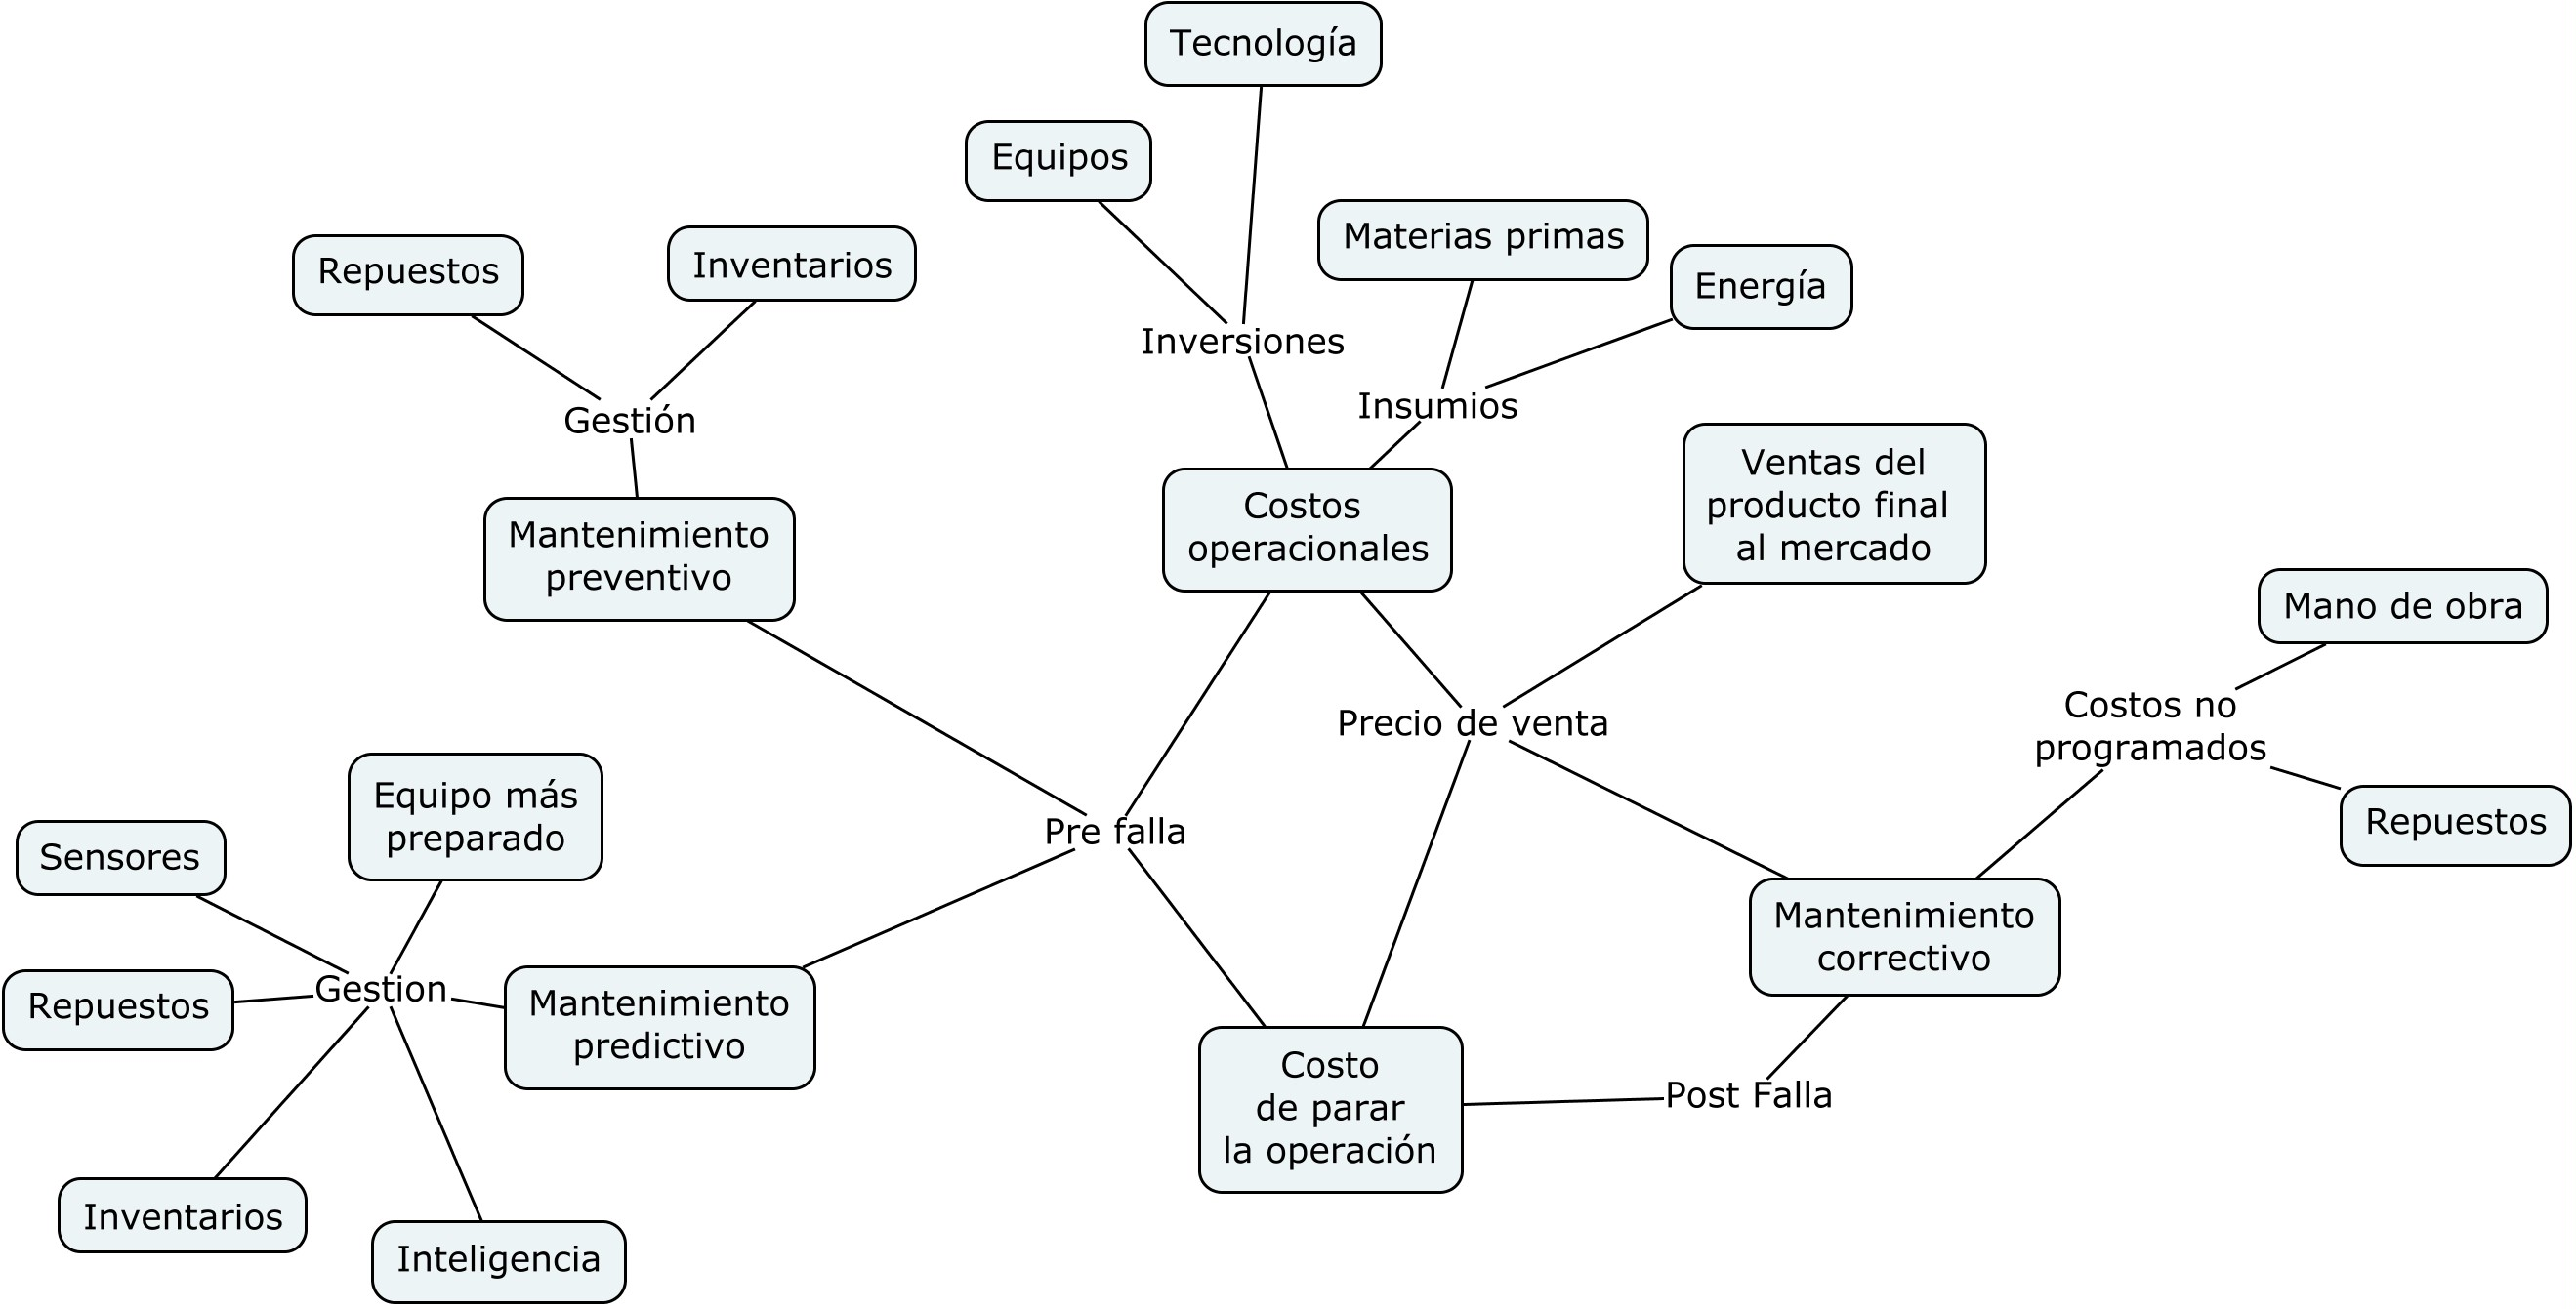
\includegraphics[scale=0.15]{Images/DURAN.jpg}
\centering
\caption{Mini modelo operación - tipos de mantenimiento}
\label{duran}
\end{figure}


\subsection{Un modelo global o por equipo}

Otra pregunta de investigación que podría plantear la presentación del profesor Duran, dice relación con los modelos más genéricos, estos modelos tienen la ventaja de describir con precisión comportamientos en el largo plazo, pero podríamos asumir que para el tomador final de decisiones estos modelos no proporcionan el total de la información requerida.

Un modelo por equipos, por ejemplo "Molino SAG", necesariamente entregaría información mas detallada y adecuada para la operación, pero, los costos asociados a esta investigación científica aplicada (toma de datos, estadística, escasa replicabilidad, poco impacto en revistas), son muy altos en términos académicos.

La alternativa que acá se abre es la relación Universidad - Empresa y como esta interacción apoya a los ingenieros de terreno en su gestión y en la gestión global de los costos.

\subsection{Un modelo continuo (una propuesta)}

Una propuesta final, y quizás que presenta más desviaciones con lo real, es la de plantear los sistemas como continuos y asumir los costos como variables durante el tiempo.

Asumir esto, en el caso de estar correcto, cobraría importancia al poder analizar la interdependencia de los costos de mantener con otros costos importantes y de peso, como por ejemplo los costos de la energía (no es descabellado pensar que si un lubricante no esta en condiciones adecuadas, mucha energía se disipará en forma de calor, por ejemplo).

\begin{equation}
c\frac{\partial C_{mt}}{\partial t} =  \frac{\partial (\frac{\partial C_{mcr}}{\partial t}+\frac{\partial C_{mpr}}{\partial t}+\frac{\partial C_{mpv}}{\partial t})}{\partial E}+S
\end{equation}

Donde:

\begin{itemize}
    \item $C_{mt}$: Costo total de mantener.
    \item $C_{mcr}$: Costo del mantenimiento correctivo.
    \item $C_{mpr}$: Costo del mantenimiento predictivo.
    \item $E$: Costo de la energía.
    \item $c$: Constante de proporcionalidad para el modelo.
    \item $S$: Costos fijos.
\end{itemize}

Un modelo así requeriría gran capacidad de cálculo para la resolución por métodos numéricos (de tener ecuaciones que lo sustenten), pero podría presentar volúmenes o mapas de calor útiles para cuantificar las interrelaciones propuestas.

\nocite{*}
    \bibliography{src/ref}

\end{document}
